\documentclass{article}

% Recommended, but optional, packages for figures and better typesetting:
% \usepackage{subfigure}

\usepackage{booktabs}       % professional-quality tables
\usepackage{amsfonts}       % blackboard math symbols
\usepackage{nicefrac}       % compact symbols for 1/2, etc.
\usepackage{microtype}      % microtypography
\usepackage{graphicx}
\usepackage{multirow}
\usepackage{amsmath}
\usepackage{amssymb}
\usepackage{subcaption}
\usepackage{paralist}
\usepackage{tabularx}
\usepackage{xcolor}
\usepackage[noend]{algpseudocode}
\usepackage{setspace}
\usepackage{enumitem}
% operators

\newcommand{\argmax}{\operatornamewithlimits{argmax}}
\newcommand{\argmin}{\operatornamewithlimits{argmin}}

% vectors
\let\avec\vec
%\renewcommand{\vec}[1]{\ensuremath{\boldsymbol{#1}}}
\renewcommand{\v}[1]{\ensuremath{\boldsymbol{#1}}}

\newcommand{\src}{\lstinline[mathescape, keepspaces]}
\newcommand{\msrc}[1]{\mbox{\src!#1!}}

\newcommand{\tens}[1]{%
  \mathbin{\mathop{\otimes}\limits_{#1}}%
}

% symbol shorthands (lowercase)
%\newcommand{\x}{\ensuremath{\v{x}}}
%\newcommand{\y}{\ensuremath{\v{y}}}
%\newcommand{\z}{\ensuremath{\v{z}}}
%\newcommand{\h}{\v{\eta}}
%\newcommand{\e}{\v{\epsilon}}
%\renewcommand{\u}{\v{u}}
\newcommand{\pd}{\ensuremath{\partial}}
\newcommand{\x}{\ensuremath{x}}
\newcommand{\y}{\ensuremath{y}}
\newcommand{\z}{\ensuremath{z}}
\newcommand{\h}{\ensuremath{\eta}}
\newcommand{\e}{\ensuremath{\epsilon}}
\renewcommand{\u}{\ensuremath{u}}
\newcommand{\q}{\theta}
\newcommand{\f}{\phi}
\renewcommand{\l}{\lambda}
\renewcommand{\t}{\tau}

% symbol shorthands (uppercase)
\renewcommand{\L}{\ensuremath{\mathcal{L}}}
\newcommand{\KL}[2]{\ensuremath{\mathrm{KL}\left({#1} \:\middle\vert\middle\vert\: {#2}\right)}}
\newcommand{\E}{\ensuremath{\mathbb{E}}}
\newcommand{\N}{\ensuremath{\mathcal{N}}}
\newcommand{\C}{\ensuremath{\mathtt{Concrete}}}

%\let\lmid\mid
%\renewcommand{\mid}{\!\lmid\!}

\newcommand{\eval}{\ensuremath{$\reflectbox{$\,\leadsto\,$}$}}
%\newcommand{\eval}{\sim}
\newcommand{\hide}[1]{}

\makeatletter
\DeclareRobustCommand{\cev}[1]{%
  \mathpalette\do@cev{#1}%
}
\newcommand{\do@cev}[2]{%
  \fix@cev{#1}{+}%
  \reflectbox{$\m@th#1\vec{\reflectbox{$\fix@cev{#1}{-}\m@th#1#2\fix@cev{#1}{+}$}}$}%
  \fix@cev{#1}{-}%
}
\newcommand{\fix@cev}[2]{%
  \ifx#1\displaystyle
    \mkern#23mu
  \else
    \ifx#1\textstyle
      \mkern#23mu
    \else
      \ifx#1\scriptstyle
        \mkern#22mu
      \else
        \mkern#22mu
      \fi
    \fi
  \fi
}


\definecolor[named]{Blue}{cmyk}{1,0.1,0,0.1}
\definecolor[named]{Yellow}{cmyk}{0,0.16,1,0}
\definecolor[named]{Orange}{cmyk}{0,0.42,1,0.01}
\definecolor[named]{Red}{cmyk}{0,0.90,0.86,0}
\definecolor[named]{LightBlue}{cmyk}{0.49,0.01,0,0}
\definecolor[named]{Green}{cmyk}{0.20,0,1,0.19}
\definecolor[named]{Purple}{cmyk}{0.55,1,0,0.15}
\definecolor[named]{DarkBlue}{cmyk}{1,0.58,0,0.21}

\usepackage[acronym,smallcaps,nowarn,section,nogroupskip,nonumberlist]{glossaries}
\glsdisablehyper{}
\newacronym{SCFM}{scfm}{stochastic control-flow model}
\newacronym{WS}{ws}{wake-sleep}
\newacronym{BWS}{bws}{basic wake-sleep}
\newacronym{RWS}{rws}{reweighted wake-sleep}
\newacronym{ELBO}{elbo}{evidence lower bound}
\newacronym{VAE}{vae}{variational autoencoder}
\newacronym{IWAE}{iwae}{importance weighted autoencoder}
\newacronym{KL}{kl}{Kullback-Leibler}
\newacronym{SGD}{sgd}{stochastic gradient descent}
\newacronym{VIMCO}{vimco}{variational inference for Monte Carlo objectives}
\newacronym{WW}{ww}{wake-wake}
\newacronym{WWS}{wws}{wake-wake-sleep}
\newacronym{AIR}{air}{Attend, Infer, Repeat}
\newacronym{ESS}{ess}{effective sample size}
\newacronym{REINFORCE}{reinforce}{Reinforce gradient estimator}
\newacronym{IS}{is}{importance sampling}
\newacronym{GMM}{gmm}{Gaussian mixture model}
\newacronym{MNIST}{mnist}{hand-written digit dataset}
\newacronym{RELAX}{relax}{RELAX gradient estimator}
\newacronym{REBAR}{rebar}{REBAR gradient estimator}
\newacronym{PMF}{pmf}{probability mass function}
\newacronym{MLP}{mlp}{multilayer perceptron}
\newacronym{RNN}{rnn}{recurrent neural network}
\newacronym{PCFG}{pcfg}{probabilistic context free grammar}
\newacronym{ADAM}{adam}{ADAM}
\glsunset{ADAM}

\usepackage{amsthm}
\newtheorem{proposition}{Proposition}
\theoremstyle{definition}
\newtheorem{definition}{Definition}

\newcommand{\given}{\lvert}
\newcommand{\pw}{\overset{\text{p.w.}}{\sim}
}
%%%%%%% hand-added %%%%%


% hyperref makes hyperlinks in the resulting PDF.
% If your build breaks (sometimes temporarily if a hyperlink spans a page)
% please comment out the following usepackage line and replace
% \usepackage{icml2020} with \usepackage[nohyperref]{icml2020} above.
\usepackage{hyperref}

% Attempt to make hyperref and algorithmic work together better:
\newcommand{\theHalgorithm}{\arabic{algorithm}}

% Use the following line for the initial blind version submitted for review:
\usepackage{icml2020}

% If accepted, instead use the following line for the camera-ready submission:
% \usepackage[accepted]{icml2020}

% The \icmltitle you define below is probably too long as a header.
% Therefore, a short form for the running title is supplied here:
\icmltitlerunning{Amortized Population Gibbs Samplers with Neural Sufficient Statistics}

\begin{document}
\appendix

\onecolumn
\icmltitle{Supplementary Material: Amortized Population Gibbs Samplers with Neural Sufficient Statistics}
\icmlkeywords{Machine Learning, ICML}
\vskip 0.3in


\section{Gradient of the generative model}% $p_\q(x \mid z)$}
\label{appendix:grad-theta}
This is actually a known (although indeed not obvious) identity. Briefly, we can express the expected gradient of the log joint as
\begin{align*}
    \mathbb{E}_{p_\q(\z | \x)} 
    \left[
    \nabla_\q \log p_\q(\x, \z)
    \right]
    \mathbb{E}_{p_\q(\z | \x)} 
    \left[
    \nabla_\q \log p_\q(\x) + \nabla_\q \log p_\q(\z | \x)
    \right]
    \mathbb{E}_{p_\q(\z | \x)} 
    \left[
    \nabla_\q \log p_\q(\x) 
    \right]
    \nabla_\q \log p_\q(\x)
\end{align*}
Here we make use of a standard identity that is also used in, e.g., likelihood-ratio estimators
\begin{align*}
\mathbb{E}_{p_\q(\z | \x)}
\left[
    \nabla_\q \log p_\q(\z | \x)
\right] 
=
\int p_\q(\z | \x) \nabla_\q \log p_\q(\z | \x) \: dz
=
\int \nabla_\q p_\q(\z | \x) \: dz
=
\nabla_\q \int p_\q(\z | \x) \: dz
=
\nabla_\q 1
= 
0
\end{align*}
Therefore, we have the the following equality
\begin{align*}
\nabla_\q \log p_\q(\x) 
= 
\mathbb{E}_{p_\q(\z | \x)} 
\left[
\nabla_\q \log p_\q(\x, \z)
\right].
\end{align*}
which is Equation ~\ref{eq:grad-theta}. As a result, we can then use self-normalized importance sampling to approximate     $\mathbb{E}_{p_\q(\z | \x)} \left[\nabla_\q \log p_\q(\x, \z) \right]$.

\section{Importance weights in sequential importance sampling}
\label{appendix:sis-weight}
At step $k=1$, we use exactly the standard importance sampler, thus it is obvious that the following is a valid importance weight
\begin{align*}
    w^1 = \frac{\gamma^1(z^1)}{q^1(z^1)}.
\end{align*}
When step $k>2$, we are going to prove that the importance weight relative to the intermediate densities has the form
\begin{align}
    \label{appendix:eq:sis-weight}
    w^k
    = 
    \frac{\gamma^k(z^{1:k})}
         {q^1(z^1) \prod_{k'=2}^k q^{k'}(z^{k'} \mid z^{1:k'-1})}.
\end{align}

At step $k=2$, the importance weight is defined as 
\begin{align*}
    w^k 
    &= 
    v^{2} \: w^1
    \: =
    \frac{\gamma^2(z^{1:2})}{\gamma^{1}(z^{1})\:q^2(z^2 \mid z^{1})} \frac{\gamma^1(z^1)}{q^1(z^1)}
    \: = \frac{\gamma^2(z^{1:2})}{q^1(z^1) \: q^2(z^2 \mid z^{1})}.
\end{align*}
which is exactly that form. Now we prove weights in future steps by induction. At step $k\geq 2$, assume the weight has the form in Equation~\ref{appendix:eq:sis-weight}, i.e.
\begin{align*}
    w^k
    = 
    \frac{\gamma^k(z^{1:k})}
         {q^1(z^1) \prod_{k'=2}^k q^{k'}(z^{k'} \mid z^{1:k'-1})}.    
\end{align*}
, then at step $k+1$, the importance weight is the product of incremental weight and incoming weight 
\begin{align*}
    w^{k+1}
    =
    v^{k+1} \: w^k
    =
    \frac{\gamma^{k+1}(z^{1:k+1})}{\gamma^{k}(z^{1:k})\:q^{k+1}(z^{k+1} \mid z^{1:k})}
    \frac{\gamma^k(z^{1:k})}
         {q^1(z^1) \prod_{k'=2}^k q^{k'}(z^{k'} \mid z^{1:k'-1})}
    =
    \frac{\gamma^{k+1}(z^{1:k+1})}{q^1(z^1) \prod_{k'=2}^{k+1} q^{k'}(z^{k'} \mid z^{1:k'-1})}
    .    
\end{align*}
Thus the importance weight $w^k$ has the form of Equation~\ref{appendix:eq:sis-weight} at each step $k>2$ in sequential importance sampling.
\section{ Derivation of Posterior Invariance}
\label{appendix:posterior-invariance}
We can see that individual block updates leave the posterior invariant by proposing variables $\z^k_{\preceq b}$ from a partial kernel $\kappa(\z^k_{\preceq b} \mid x, \z^{k-1})$ and then marginalize over the corresponding variables from the previous step $\z^{k-1}_{\preceq b}$,
\begin{align*}
    \int 
    dz^{k-1}_{\preceq b} 
    \:
    p_\q(\z^{k-1} \mid \x) 
    \: 
    \kappa(\z^k_{\preceq b} \mid x, \z^{k-1}) 
    %\\
    %&= 
    &=
    \int 
    dz^{k-1}_{\preceq b} 
    \:
    p_\q(\z^{k-1} \mid \x) 
    \: 
    \int dz^k_{\succ b}
    \:
    \kappa(\z^k \mid x, \z^{k-1})
    \\
    &= 
    \int 
    dz^{k-1}_{\preceq b} 
    \: 
    p_\q(\z^{k-1} \mid x)
    \prod_{m=1}^b p_\q(\z^k_m \mid \x, \z^{k}_{\prec m}, \z^{k-1}_{\succ m})
    \\
    &=
    \int 
    dz^{k-1}_{\preceq b} 
    \: 
    p_\q(\z^{k-1} \mid \x)
    p_\q(\z^k_{\preceq b} \mid \x, \z^{k-1}_{\succ 1})
    \\
    %&=
    %\int d\z^{k-1}_{\preceq b} 
    %\: p_\q(\z^k_{\preceq b}, \z^{k-1} \mid \x)\\
    &=
    p_\q(\z^k_{\preceq b}\:, \: \z^{k-1}_{\succ b} \mid \x)
    .
\end{align*}

\section{Proof of the amortized population Gibbs algorithm}
\label{appendix:proof-algo}

Here, we provide an alternative proof of correctness of the APG algorithm given in Algorithm~\ref{alg:amortized-gibbs}, based on the construction of proper weights~\cite{naesseth2015nested} which was introduced after SMC samplers~\cite{delmoral2006sequential}.
We first introduce proper weights, and then present several operations that preserve the proper weighting property and finally we apply these properties in proving correctness of APG.

\subsection{Proper weights}

\begin{definition}[Proper weights]
    Given an unnormalized density $\tilde p(z)$, with corresponding normalizing constant $Z_p := \int \tilde p(z) \,\mathrm dz$ and normalized density $p \equiv \tilde p / Z_p$, the random variables $z, w \sim P(z, w)$ are properly weighted with respect to $\tilde p(z)$ if and only if for any measurable function $f$
    \begin{align}
    \label{eq:pw}
    \E_{P(z, w)}\left[w f(z)\right] = Z_p \E_{p(z)}[f(z)]. 
    \end{align}
    We will also denote this as
    \begin{align*}
        z, w \pw \tilde p.
    \end{align*}
\end{definition}

\paragraph{Using proper weights.}
Given independent samples $z^l, w^l \sim P$, we can estimate $Z_p$ by setting $f \equiv 1$:
\begin{align*}
    Z_p \approx \frac{1}{L} \sum_{l = 1}^L w^l.
\end{align*}
This estimator is unbiased because it is a Monte Carlo estimator of the left hand side of \eqref{eq:pw}.
We can also estimate $\E_{p(z)}[f(z)]$ as
\begin{align*}
    \E_{p(z)}[f(z)] \approx \frac{\frac{1}{L} \sum_{l = 1}^L w^l f(z^l)}{\frac{1}{L} \sum_{l = 1}^L w^l}.
\end{align*}
While the numerator and the denominator are unbiased estimators of $Z_p \E_{p(z)}[f(z)]$ and $Z_p$ respectively, their fraction is biased.
We often write this estimator as
\begin{align}
    \E_{p(z)}[f(z)] \approx \sum_{l = 1}^L \bar w^l f(z^l), \label{eq:pw-estimation}
\end{align}
where $\bar w^l := w^l / \sum_{l' = 1}^L w^{l'}$ is the normalized weight.

\subsection{Operations that preserve proper weights}


\begin{proposition}[Nested importance sampling]
    Adapted from \cite[Algorithm 1]{naesseth2015nested}.
    Given unnormalized densities $\tilde q(z), \tilde p(z)$ with the normalizing constants $Z_q, Z_p$ and normalized densities $q(z), p(z)$, if 
    \begin{align}
        z, w \pw \tilde q, \label{eq:1}
    \end{align}
    then
    \begin{align*}
        z, \frac{w\tilde p(z)}{\tilde q(z)} \pw \tilde p.
    \end{align*}
\end{proposition}
\begin{proof}
    First define the distribution of $z, w$ as $Q$.
    For measurable $f(z)$
    \begin{align*}
        \E_{Q(z, w)}\left[\frac{w\tilde p(z)}{\tilde q(z)} f(z)\right] 
        = Z_q \E_{q(z)}\left[\frac{\tilde p(z) f(z)}{\tilde q(z)}\right]
        = Z_q \int q(z) \frac{\tilde p(z) f(z)}{\tilde q(z)} \,\mathrm dz
        = \int \tilde p\textbf{}(z) f(z) \,\mathrm dz
        = Z_p \E_{p(z)}[f(z)].
    \end{align*}
\end{proof}



\begin{proposition}[Resampling]
\label{proposition:resampling}
    Adapted from \cite[Section 3.1]{naesseth2015nested}.
    Given an unnormalized density $\tilde p(z)$ (normalizing constant $Z_p$, normalized density $p(z)$), if we have a set of properly weighted samples
    \begin{align}
        z^l, w^l \pw \tilde p,  \quad l = 1,\ldots, L \label{eq:bla}
    \end{align}
    then the resampling operation preserves the proper weighting, i.e.
    \begin{align*}
        z'^{\:l}, w'^{\:l} \pw \tilde p, \quad l = 1,\ldots, L
    \end{align*}
    where $z'^{\:l} = z^{a}$ with probability $P(a = i) = w^i / \sum_{l=1}^L w^l$ and $w'^{\:l} := \frac{1}{L} \sum_{l = 1}^L w^l$.
\end{proposition}
\begin{proof}
    Define the distribution of $z^l, w^l$ as $\hat{P}$.
    We show that for any $f$, $\E[f(z^{a}) w'^{\:l}] = Z_p \E_{p(z)}[f(z)]$.
    \begin{align*}
    &
        \E_{\left(\prod_{l=1}^L \hat{P}(z^l, w^l)\right) p(a \mid w^{1:L})} \bigg[f(z^{a}) w'^{l}\bigg] \\
        &= \E_{\prod_{l=1}^L \hat{P}(z^l, w^l)}\left[\sum_{i = 1}^L f(z^i) w' \: P(a = i)\right]  \\
        &= \E_{\prod_{l=1}^L \hat{P}(z^l, w^{l})}\left[\sum_{i = 1}^L f(z^i) w'  \frac{w^i}{ \sum_{l'=1}^L w^{l'}}\right]  \\
        &= \E_{\prod_{l=1}^L \hat{P}(z^l, w^l)}\left[\frac{1}{L}\sum_{i = 1}^L f(z^i) w^i\right] \\
        &= \frac{1}{L}\sum_{i = 1}^L \E_{\hat{P}(z^i, w^i)}\left[f(z^i) w^i\right]
        = \frac{1}{L}\sum_{i = 1}^L Z_p \E_{p(z)}[f(z)]
        = Z_p \: \E_{p(z)}[f(z)]. 
    \end{align*}
\end{proof}
Therefore, the resampling will return a new set of samples that are still properly weighted relative to the target distribution in the APG sampler (Algorithm~\ref{alg:amortized-gibbs}).
\begin{proposition}[Move]
\label{proposition:extendedspace}
    Given an unnormalized density $\tilde p(z)$ (normalizing constant $Z_p$, normalized density $p(z)$) and normalized conditional densities $q(z' \given z)$ and $r(z \given z')$, the proper weighting is preserved if we apply the transition kernel to a properly weighted sample, i.e.~if we have
    \begin{align}
        &
        z^l, w^l \pw \tilde p, \label{eq:pw-of-p}\\[1em]
        &
         z'^{\:l} \sim q(z'^{\:l} \given z^l),  \label{eq:z-prime}\\[1em]
        &
        w'^{\:l} = \frac{\tilde p(z'^{\:l})r(z^l \given z'^{\:l})}{\tilde p(z^l)q(z'^{\:l} \given z^l)} w^l, \qquad l = 1, \ldots, L \label{eq:w-prime}
    \end{align}
%     \noindent\begin{subequations} 
%     \begin{tabularx}{\textwidth}{@{}XXX@{}}
%         \begin{equation}
%             z, w \pw \tilde p, \label{eq:pw-of-p}
%         \end{equation}&
%         \begin{equation}
%             z' \sim q(z' \given z), \label{eq:z-prime}
%         \end{equation}&
%         \begin{equation}
%             w' = \frac{\tilde p(z')r(z \given z')}{\tilde p(z)q(z' \given z)} w, \label{eq:w-prime}
%         \end{equation}
%     \end{tabularx}
%   \end{subequations} 
then we have
    \begin{align}
        z'^{\:l}, w'^{\:l} \pw \tilde p, \qquad  l = 1, \ldots, L \label{eq:to-prove}
    \end{align}
\end{proposition}
\begin{proof}
    Firstly we simplify the notation by dropping the superscript $l$ without loss of generality. Define the distribution of $z, w$ as $\hat{P}$.
    Then, due to \eqref{eq:pw-of-p}, for any measurable $f(z)$, we have
    \begin{align*}
        \E_P[w f(z)] = Z_p E_{p}[f(z)].
    \end{align*}
    To prove \eqref{eq:to-prove}, we show $\E_{\hat{P}(z, w)q(z' \given z)}[w' f(z')] = Z_p \E_{p(z')}[f(z')]$ for any $f$ as follows:
    \begin{align}
        \E_{\hat{P}(z, w)q(z' \given z)}[w' f(z')]
        &= \E_{\hat{P}(z, w)q(z' \given z)}\left[\frac{\tilde p(z')r(z \given z')}{\tilde p(z)q(z' \given z)} w f(z')\right] 
        \nonumber\\
        &= \int \hat{P}(z, w)q(z' \given z) \frac{\tilde p(z')r(z \given z')}{\tilde p(z)q(z' \given z)} w f(z') \,\mathrm dz \,\mathrm dw \,\mathrm dz' 
        \nonumber\\
        &= \int \hat{P}(z, w) \frac{\tilde p(z')r(z \given z')}{\tilde p(z)} w f(z') \,\mathrm dz \,\mathrm dw \,\mathrm dz' 
        \nonumber\\
        &= \int \tilde p(z') f(z') \left(\int \hat{P}(z, w) w \frac{r(z \given z')}{\tilde p(z)}\,\mathrm dz \,\mathrm dw\right) \,\mathrm dz'
        \nonumber\\
        &= \int \tilde p(z') f(z') Z_p \E_{p(z)}\left[\frac{r(z \given z')}{\tilde p(z)}\right] \,\mathrm dz'. \label{eq:pause}
    \end{align}
    Using the fact that $\E_{p(z)}\left[\frac{r(z \given z')}{\tilde p(z)}\right] = \int p(z) \frac{r(z \given z')}{\tilde p(z)} \,\mathrm dz = \int r(z \given z') \,\mathrm dz / Z_p = 1 / Z_p$.
    Equation~\ref{eq:pause} simplifies to
    \begin{align*}
        \int \tilde p(z') f(z') \,\mathrm dz' = Z_p \E_{p(z')}[f(z')].
    \end{align*}
\end{proof}

\subsection{Correctness of APG Sampler}
We provide the proof by performing 2 steps in the APG sampler (Algorithm~\ref{alg:amortized-gibbs}), i.e,~ we prove the correctness when we initialize samples at step $k=1$ (line~\ref{line:rws-loop} - line~\ref{line:rws-grad-theta}) and then do one Gibbs sweep at step $k=2$ (line~\ref{line:apg-sweep-begin} - line~\ref{line:apg-sweep-end}). In fact, its correctness still holds if we perform more Gibbs sweeps by induction.

\textbf{Step $k=1$}. We initialize the proposal $z\sim q_\phi(z \given x)$ (line~\ref{line:rws-propose}) and train that encoder using the wake-$\phi$ phase objective in the standard reweighted wake-sleep\cite{le2019revisiting}
$\E_{p(x)}\left[\textsc{kl}\left(p_\theta(z \given x) || q_\phi(z \given x)\right)\right]$. 
Then we estimate its gradient w.r.t. parameter $\phi$ (line~\ref{line:rws-grad-phi}) as
\begin{align}
    \label{eq:g-rws-phi}
    g_\phi :&= - \nabla_\phi \: \E_{p(x)}\left[\textsc{kl}\left(p_\theta(z \given x) || q_\phi(z \given x)\right)\right] \\
    &
    =
    \E_{p(x)}\left[
    \E_{p_\theta(z \given x)}\left[\nabla_\phi \log q_\phi(z \mid x)\right]
    \right]
    . 
\end{align}

\textbf{Step $k=2$}. After one full sweep, we have the following objective
\begin{align*}
    \E_{p(x)}\Big[
    \sum_{b = 1}^B\E_{p_\theta(z_{-b} \mid x)}\left[\textsc{kl}\left(p_\theta(z_b \mid z_{-b}, x) || q_\phi(z_b \mid x, z_{-b})\right)\right]\Big] 
\end{align*}


% Then we estimate the gradient of the following objective after $K$ sweeps
% \begin{align}
%     \mathcal K(\phi) :=  \E_{p(x)}\Big[\textsc{kl}\left(p_\theta(z_{1:B} \mid x) || q_\phi(z_{1:B} \mid x)\right) 
%     + 
%     \sum_{b = 1}^B\E_{p_\theta(z_{-b} \mid x)}\left[\textsc{kl}\left(p_\theta(z_b \mid z_{-b}, x) || q_\phi(z_b \mid x, z_{-b})\right)\right]\Big] \label{eq:objective}
% \end{align}
% The first term learns an initial proposal $q_\phi(z \given x)$ and the second term (sum over $B$ terms) learns the $B$ conditionals $q_\phi(z_b \mid x, z_{-b})$.

% At the beginning of the APG algorithm, we initialize the gradient estimator $g_\f = 0$. At step $k=1$, i.e. the reweighed wake-sleep 

% line~\ref{line:rws-grad-phi}, $g_\phi$ estimates $\nabla_\phi \E_{p(x)}\left[\textsc{kl}\left(p_\theta(z_{1:B} \given x) || q_\phi(z_{1:B} \given x)\right)\right]$ as in a standard reweighted wake-sleep objective.

And we will prove that we correctly estimate the following gradient w.r.t. parameter $\phi$ at each block update (line~\ref{line:apg-grad-phi}) 
\begin{align}
    g_\phi^b 
    :&= - \nabla_\phi \E_{p(x)}\left[ \E_{p_\theta(z_{-b} \given x)}\left[\textsc{kl}\left(p_\theta(z_b \given z_{-b}, x) || q_\phi(z_b \given z_{-b}, x)\right)\right]
    \right]
    \\
%    &= \E_{p_\theta(z_{-b} \given x)}\left[\E_{p_\theta(z_b \given z_{-b}, x)}\left[  -\nabla_\phi \log q_\phi(z_b \given z_{-b}, x)\right]\right] \nonumber\\
    &= 
    \E_{p(x)}\left[
    \E_{p_\theta(z_{1:B} \given x)}\left[\nabla_\phi \log q_\phi(z_b \given z_{-b}, x)\right]
    \right], \qquad b = 1, \ldots, B
    . \label{eq:g-phi-b}
\end{align}
At each step, as long as we show that samples are properly weighted
\begin{align}
    z_{1:B}^l, w^l \pw p_\theta(z_{1:B}, x), \qquad l = 1, \ldots, L.
    \label{eq:invariant}
\end{align}
Equation~\ref{eq:pw-estimation} will guarantee the validity of both gradient estimations (line~\ref{line:rws-grad-phi} and line~\ref{line:apg-grad-phi}).

At step $k=1$, samples are properly weighted because $z^l$ and $w^l$ are proposed using importance sampling (line~\ref{line:rws-weight}) where $q_\phi(z \given x)$ is the proposal density and $p_\theta(z^l, x)$ is the unnormalized target density. The resampling step (line~\ref{line:resample}) will preserve the proper weighting because of  Proposition~\ref{proposition:resampling}.

To prove that Gibbs sweep (line~\ref{line:apg-sweep-begin} - line~\ref{line:apg-sweep-end}) in the APG sampler also preserves proper weighting, we show that each block update satisfies all the 3 conditions (Equation~\ref{eq:pw-of-p}, ~\ref{eq:w-prime} and ~\ref{eq:invariant}) in Proposition~\ref{proposition:extendedspace}, by which we can conclude the samples are still properly weighted after each block update. Without loss of generality, we drop all $l$ superscripts in the rest of the proof. Before we start any block update (before line~\ref{line:apg-propose}),  we already know that samples are properly weighted, i.e.
\begin{align}
    z, w \pw p_\theta(z, x).
\end{align}
which corresponds Equation~\ref{eq:pw-of-p}. Next we define a conditional distribution $q(z' \mid z):= q_\phi(z_b' \given x, z_{-b}) \delta_{z_{-b}}(z_{-b}')$, from which we propose a new sample
\begin{align}
    z' \sim q_\phi(z_b' \given x, z_{-b}) \delta_{z_{-b}}(z_{-b}'),
\end{align}
where the density of $z_{-b}'$ is a delta mass on $z_{-b}$ defined as $\delta_{z_{-b}}(z_{-b}') = 1$ if $z_{-b} = z_{-b}'$ and $0$ otherwise.
In fact, this sampling step is equivalent to firstly sampling $z_b' \sim q_\phi(\cdot \given x, z_{-b})$ (line~\ref{line:apg-propose}) and let $z_{-b}' = z_{-b}$, which is exactly what the APG sampler assumes procedurally. This condition corresponds to Equation~\ref{eq:z-prime}.

Finally, we define the weight $w'$
\begin{align}
    w' = \frac{{\color{blue}p_\theta(x, z_b', z_{-b}')} {\color{red}r(z_b \given x, z_{-b}) \delta_{z_{-b}}(z_{-b})}}{{\color{red}p_\theta(x, z_b, z_{-b})} {\color{blue}q_\phi(z_b' \given x, z_{-b}) \delta_{z_{-b}}(z_{-b}')}} w,
\end{align}
where the terms in blue are treated as densities (normalized or unnormalized) of $z_{1:B}'$ and the terms in red are treated as densities of $z_{1:B}$.
Since both delta mass densities evaluate to one, this weight is equal to the weight computed after each block update (line~\ref{line:apg-weight}). This condition corresponds to Equation~\ref{eq:w-prime}.

Now we can apply the conclusion \eqref{eq:to-prove} in Proposition~\ref{proposition:extendedspace} and claim 
\begin{align*}
z_{1:B}', w' \pw p_\theta(z_{1:B}', x)
.
\end{align*}
since $z_{-b} = z_{-b}'$ and $z_b = z_b'$ due to the re-assignment (line~\ref{line:apg-reassign}). Based on the fact that proper weighting is preserves at both initial step $k=1$ and the Gibbs sweep $k=2$, we have proved that both gradient estimations (line~\ref{line:rws-grad-phi} and line~\ref{line:apg-grad-phi}) are correct.

\section{Architecture of the Amortized Population Gibbs samplers}
\label{appendix:architecture}
\subsubsection*{GMM}
\begin{table}[H]
    \centering
    \begin{tabular}{c|c|c}
    \toprule
     Layer 
     & 
    \multicolumn{2}{c}{$q_\f(\mu, \tau | x)$}
    \\
    \midrule
    Input
    & 
    \multicolumn{2}{c}{$\mathrm{Concat}[x_n\in\mathbb{R}^2]$}
    \\
    \hline
    1
    & \parbox{3cm}{\centering FC 2}
    & \parbox{3cm}{\centering FC 3 Softmax}
    \\
    \bottomrule
    \end{tabular}
    \label{arch-gmm-rws}
\end{table}

\begin{table}[h!]
    \centering
    \begin{tabular}{c|c|c}
    \toprule
     Layer 
     & 
    \multicolumn{2}{c}{$q_\f(\mu, \tau | x, c)$}
    \\
    \midrule
    Input
    & 
    \multicolumn{2}{c}{$\mathrm{Concat}[x_n\in\mathbb{R}^2, c_n\in\mathbb{R}^3]$}
    \\
    \hline
    1
    & \parbox{3cm}{\centering FC 2}
    & \parbox{3cm}{\centering FC 3 Softmax}
    \\
    \bottomrule
    \end{tabular}
    \label{arch-gmm-global}
\end{table}

\begin{table}[h!]
    \centering
    \begin{tabular}{c|c}
    \toprule
        Layer
        &
        $q_\f(c | x, \mu, \tau)$
        \\
    \midrule
    Input
    & 
    $\mathrm{Concat}[x_n\in\mathbb{R}^2, \mu_i\in\mathbb{R}^2]$\\
    \hline
    1
    & \parbox{4cm}{\centering FC 32 Tanh}\\
    \hline
    2 
    & FC 1, Intermediate Variable $o_i\in\mathbb{R}$ \\
    \hline
    3
    & $\mathrm{Concat}[o_i\in\mathbb{R}]$, Softmax ($c_n$) \\
    \bottomrule
    \end{tabular}
    \label{arch-gmm-local}
\end{table}
\subsubsection*{DGMM}
\begin{table}[h!]
    \centering
    \begin{tabular}{c|c|c}
    \toprule
        \textbf{Layer} &\multicolumn{2}{c}{$q_\f(\mu | x)$} \\
    \midrule
    Input &\multicolumn{2}{c}{$x_n\in\mathbb{R}^2$} \\
    \hline
    1 
    & 
     \parbox{4cm}{\centering FC 32 Tanh}
    & 
    \parbox{4cm}{\centering FC 32 Tanh}\\
    \hline
    2 
    &
    \parbox{4cm}{\centering FC 16 Tanh, $v_n\in\mathbb{R}$}
    & 
    \parbox{4cm}{\centering FC 4 Softmax, $\gamma_n\in\mathbb{R}^{3}$}\\
    \hline
    3 &\multicolumn{2}{c}{$T_n := \gamma_n \tens{} v_n\in\mathbb{R}^{3\times16}$} \\
    \hline
    4 &\multicolumn{2}{c}{$\mathrm{Concat}[\sum_n^N T_n[i], \mu_0\in\mathbb{R}^2, \mathrm{Diag}(\sigma_0^2 I)\in\mathbb{R}^2], i=1,2,3,4$} \\
    \hline
    5 &\multicolumn{2}{c}{FC 2$\times$32 Tanh} \\
    \hline
    6 &\multicolumn{2}{c}{FC 2$\times$8 ($\mu_{1:I}$)} \\
    \bottomrule
    \end{tabular}
    \label{arch-dgmm-rws}
\end{table}

\begin{table}[h!]
    \centering
    \begin{tabular}{c|c|c}
    \toprule
        \textbf{Layer} &\multicolumn{2}{c}{$q_\f(\mu | z, c)$} \\
    \midrule
    Input &\multicolumn{2}{c}{$\mathrm{Concat}[x_n\in\mathbb{R}^2, c_n\in\mathbb{R}^3]$} \\
    \hline 
    1 
    & 
    \parbox{4cm}{\centering FC 32 Tanh}
    & 
    \parbox{4cm}{\centering FC 32 Tanh} \\
    \hline 
    2 
    &
    \parbox{4cm}{\centering FC 16, $v_n\in\mathbb{R}$}
    & 
    \parbox{4cm}{\centering FC 4 Softmax, $\gamma_n\in\mathbb{R}^{3}$}
    \\
    \hline
    3 & \multicolumn{2}{c}{$T_n := \gamma_n \tens{} v_n\in\mathbb{R}^{3\times16}$}  \\
    \hline
    4 & \multicolumn{2}{c}{$\mathrm{Concat}[\sum_n^N T_n[i], \mu_0\in\mathbb{R}^2, \mathrm{Diag}(\sigma_0^2 I)\in\mathbb{R}^2], i=1,2,3,4$} \\
    \hline 
    5 &\multicolumn{2}{c|}{FC 2$\times$32 Tanh} \\
    \hline
    6 &\multicolumn{2}{c|}{FC 2$\times$2 ($\mu_i$)} \\
    \bottomrule
    \end{tabular}
    \label{arch-dgmm-global}
\end{table}
\newpage
\begin{table}[H]
    \centering
    \begin{tabular}{c|c}
    \toprule
        \textbf{Layer} &
        $q_\f(c | z, \mu)$ \\
    \midrule
    Input  
    & 
    $\mathrm{Concat}[x_n\in\mathbb{R}^2, \mu_i\in\mathbb{R}^2]$\\
    \hline 
    1  
    & 
    FC 32 Tanh\\
    \hline 
    2
    & 
    \parbox{4cm}{FC 1, Intermediate Variable $o_i\in\mathbb{R}$} \\
    \hline
    3 & 
    \parbox{4cm}{$\mathrm{Concat}[o_i\in\mathbb{R}]$, Softmax ($c_n$)} \\
    \bottomrule
    \end{tabular}
    \label{arch-dgmm-assignment}
\end{table}
\begin{table}[H]
    \centering
    \begin{tabular}{c|c}
    \toprule
        \textbf{Layer} &
        $q_\f(\alpha | x, z, \mu)$ \\
    \midrule
    Input  
    & 
    $x_n - \mu_i \in\mathbb{R}^2 | z_n = i$\\
    \hline 
    1  
    & 
    FC 32 Tanh\\
    \hline 
    2
    & 
    \parbox{4cm}{FC 1 Tanh} \\
    \bottomrule
    \end{tabular}
    \label{arch-dgmm-angle}
\end{table}    
\begin{table}[h!]
    \centering
    \begin{tabular}{c|c}
    \toprule
    \textbf{Layer}
    &
    $p_q(x | \mu, c, \alpha)$ \\
    \midrule
    Input
    &
    $\mathrm{Concat}[\alpha_n, c_n]\in\mathbb{R}^5$ 
    \\
    \hline
    1
    &
    FC 32 Tanh \\
    \hline
    2
    &
    FC 2 Tanh ($\mu_n$, fixed $\sigma_\epsilon$)\\
    \bottomrule
    \end{tabular}
    \label{arch-dgmm-decoder}
\end{table}

\newpage
\subsubsection*{Bouncing MNIST}
\begin{table}[H]
\centering
\label{arch-bmnist-decoder}
\begin{tabular}{c|c}
    \toprule
    \textbf{Layer} & $p_\q(x | z^{\mathrm{what}}, z^{\mathrm{where}})$ \\
    \midrule
    Input & $z^{\mathrm{what}}_i \in\mathbb{R}^{10}$
    \\
    \hline
    1 &
    FC 200 ReLU \\
    \hline
    2 &
    FC 400 ReLU \\
    \hline
    3 & digit $d_i\in\mathbb{R}^{784}$\\
    \hline
    4 & ST($d_{i}, z^{\mathrm{where}}_{i, t}) \in\mathbb{R}^{9276}, i=1...,i, t=1...,T$ \\
    \bottomrule
\end{tabular}
\end{table}

\begin{table}[h!]
\centering
\begin{tabular}{c|c}
    \toprule
    \textbf{Layer} & $q_\f(z^{\mathrm{what}} | z^{\mathrm{where}})$ \\
    \midrule
    Input & $x_t\in\mathbb{R}^{9276}, z^{\mathrm{where}}_{i, t}\in\mathbb{R}^{2}, i=1...,I, t=1...,T$
    \\
    \hline
    1 & 
    ST($x_t$, $z^{\mathrm{where}} _{i, t}$) $\in\mathbb{R}^{784}, i=1,..,I, t=1,...,T$  \\
    \hline
    2 &
    FC 400 ReLU \\
    \hline
    3 &
    FC 200 ReLU \\
    \hline
    4 & $z^{\mathrm{what}}_{i, t} \in\mathbb{R}^{10}, i=1,..,I, t=1,...,T$  \\
    \hline
    5 &
    Mean($z^{\mathrm{what}}_{1, t}$, $1:T$) $\in\mathbb{R}^{10}, i=1,...,I$\\
    \bottomrule
    \label{arch-bmnist-enc-what}
\end{tabular}
\end{table}

\begin{table}[h!]
    \centering
    \begin{tabular}{c|c}
     \toprule
    \textbf{Layer} & $q_\f(z^{\mathrm{where}} | z^{\mathrm{what}})$ \\
    \midrule
    Input &
    $x_t\in\mathbb{R}^{9276}$, $z^{\mathrm{what}}_{i, t}, i=1,.., t=1,..,T$ \\
    \hline
    1 & 
    Conv2d($x_t$, $z^{\mathrm{what}}_{i, t}$)$\in\mathbb{R}^{4638}$, $i=1,.., t=1,..,T$ \\
    \hline
    2  &
    FC 400 Tanh \\
    \hline
    3 & $2\times$ FC 200 Tanh \\
    \hline
    4 &
    $2\times2$ Tanh 
    \\
    \bottomrule
    \end{tabular}
    \label{arch-bmnist-enc-where}
\end{table}
\newpage
\section{More Qualitative Results of Bouncing MNIST}
\label{appendix:full-recons}
The following are full reconstructions on test sets where time steps $T=100$ and number of digits $D=3, 4, 5$, respectively. In each figure, the 1st, 3rd, 5th, 7th, 9th rows show the inference results, while the other rows show the reconstruction of the series above.
\begin{figure*}[h!]
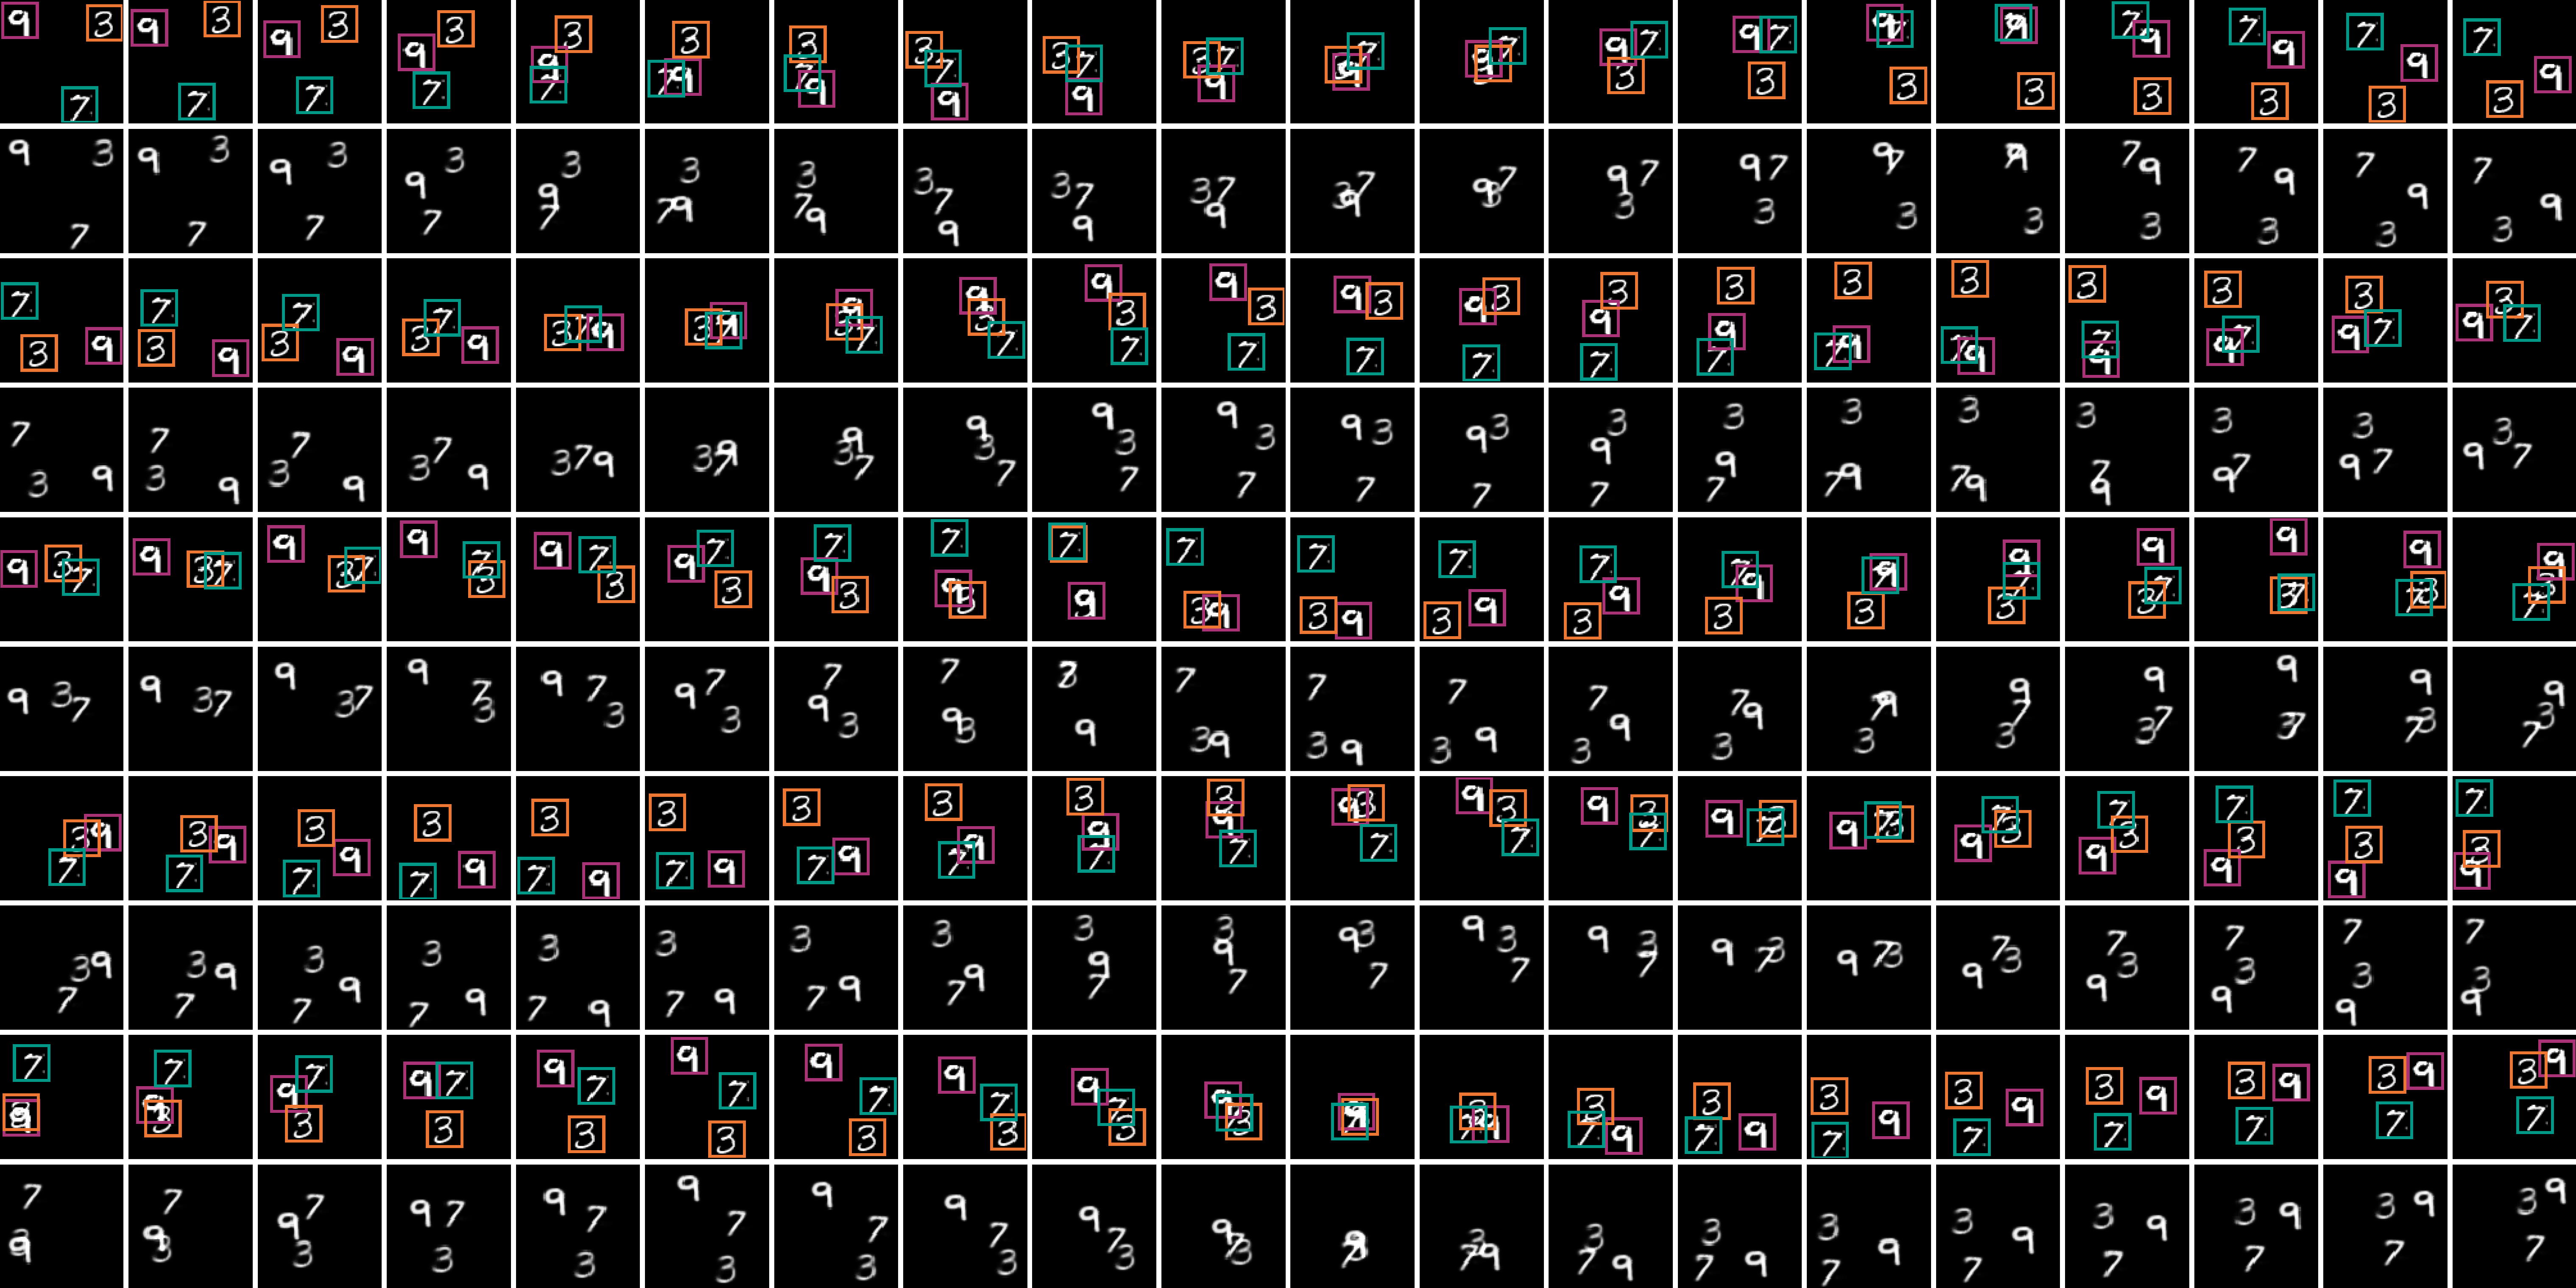
\includegraphics[width=170mm]{figures/T=100-D=3.pdf}
\caption{Full reconstruction for a video where $T=100, D=3$.}
\end{figure*}


\begin{figure*}[h!]
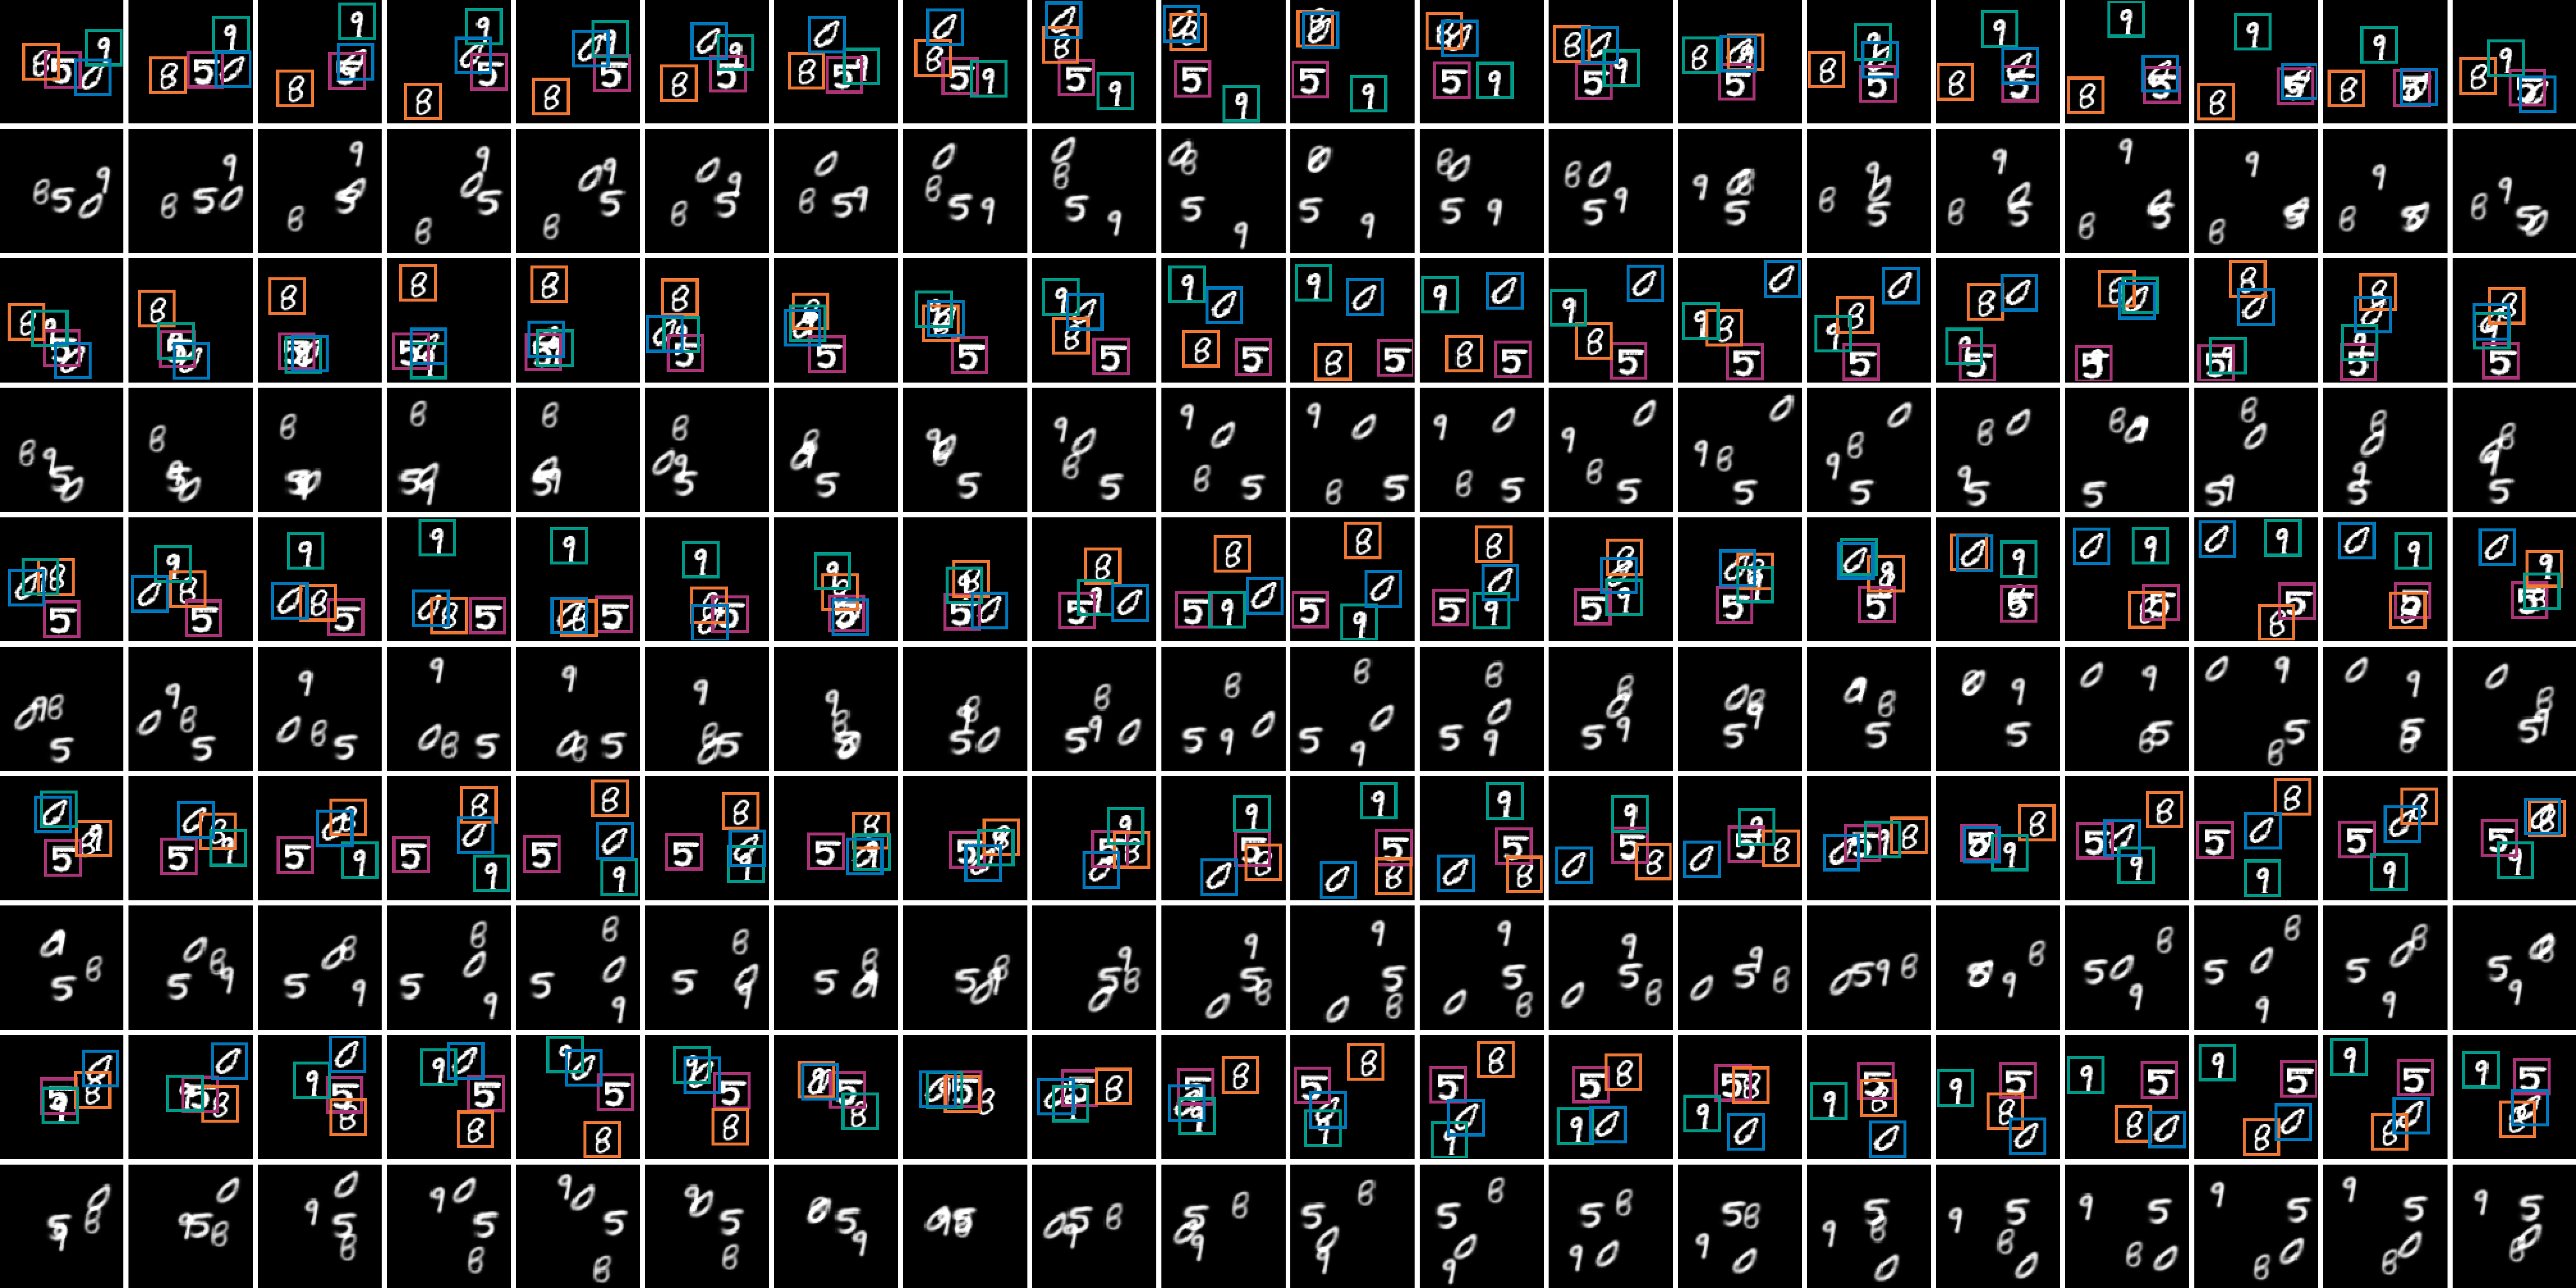
\includegraphics[width=170mm]{figures/T=100-D=4.pdf}
\caption{Full reconstruction for a video where $T=100, D=4$.}
\end{figure*}
\newpage
\begin{figure*}[h!]
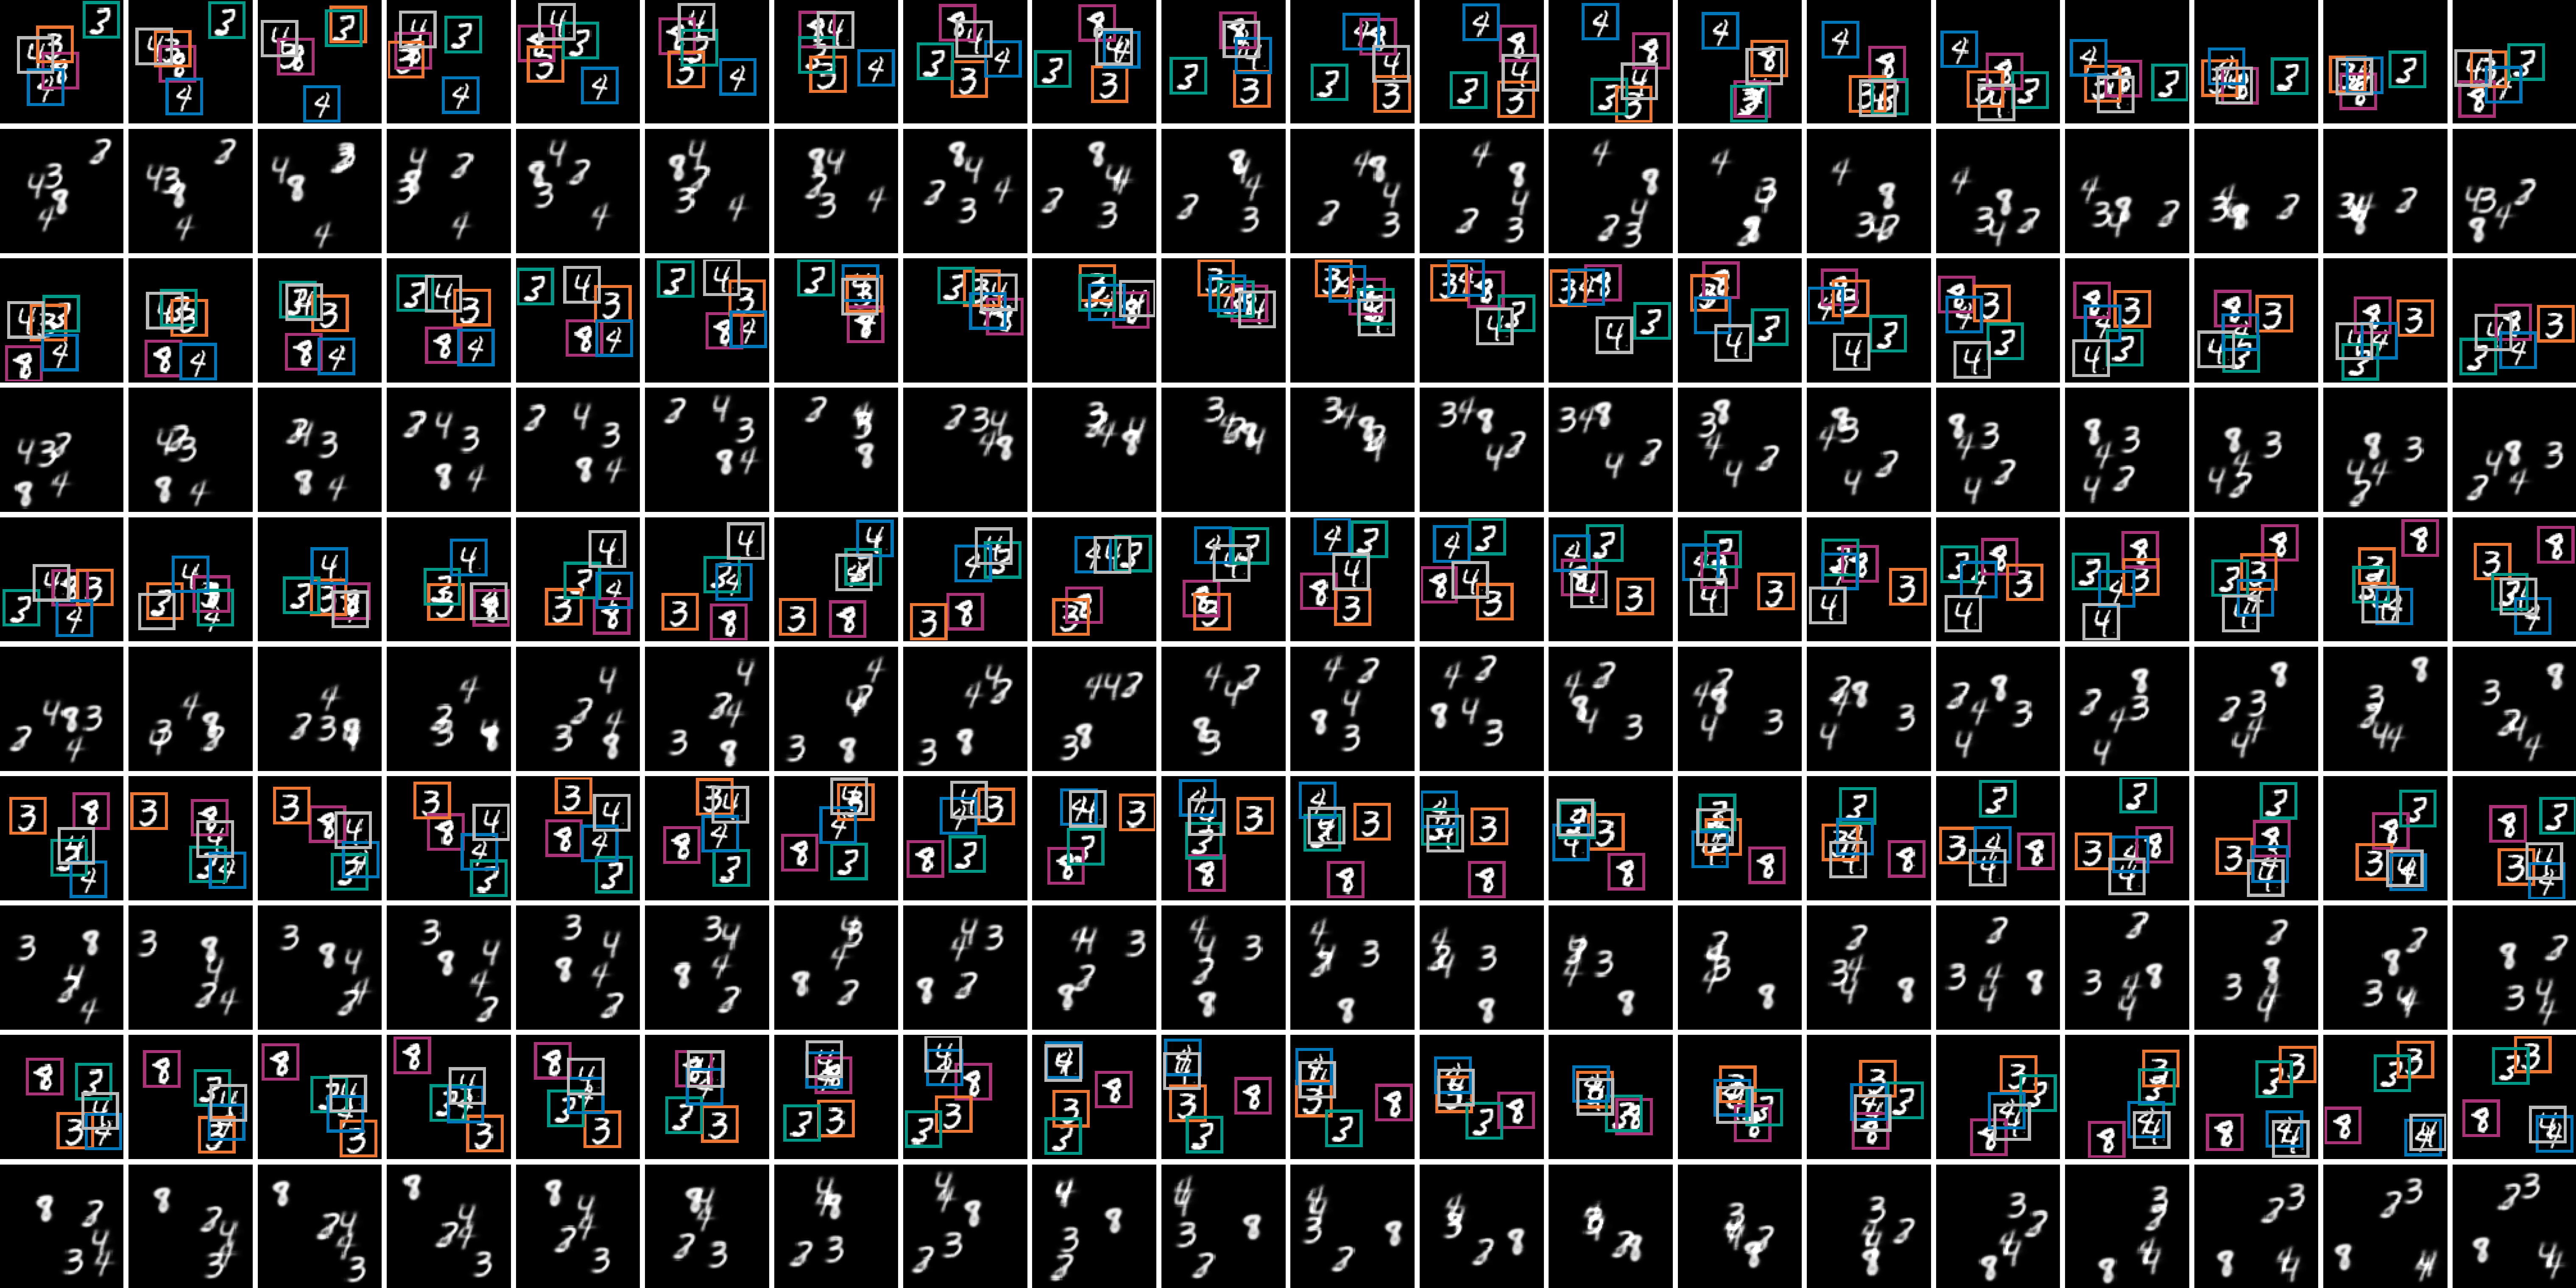
\includegraphics[width=170mm]{figures/T=100-D=5.pdf}
\caption{Full reconstruction for a video where $T=100, D=5$.}
\end{figure*}

\begin{figure*}[h!]
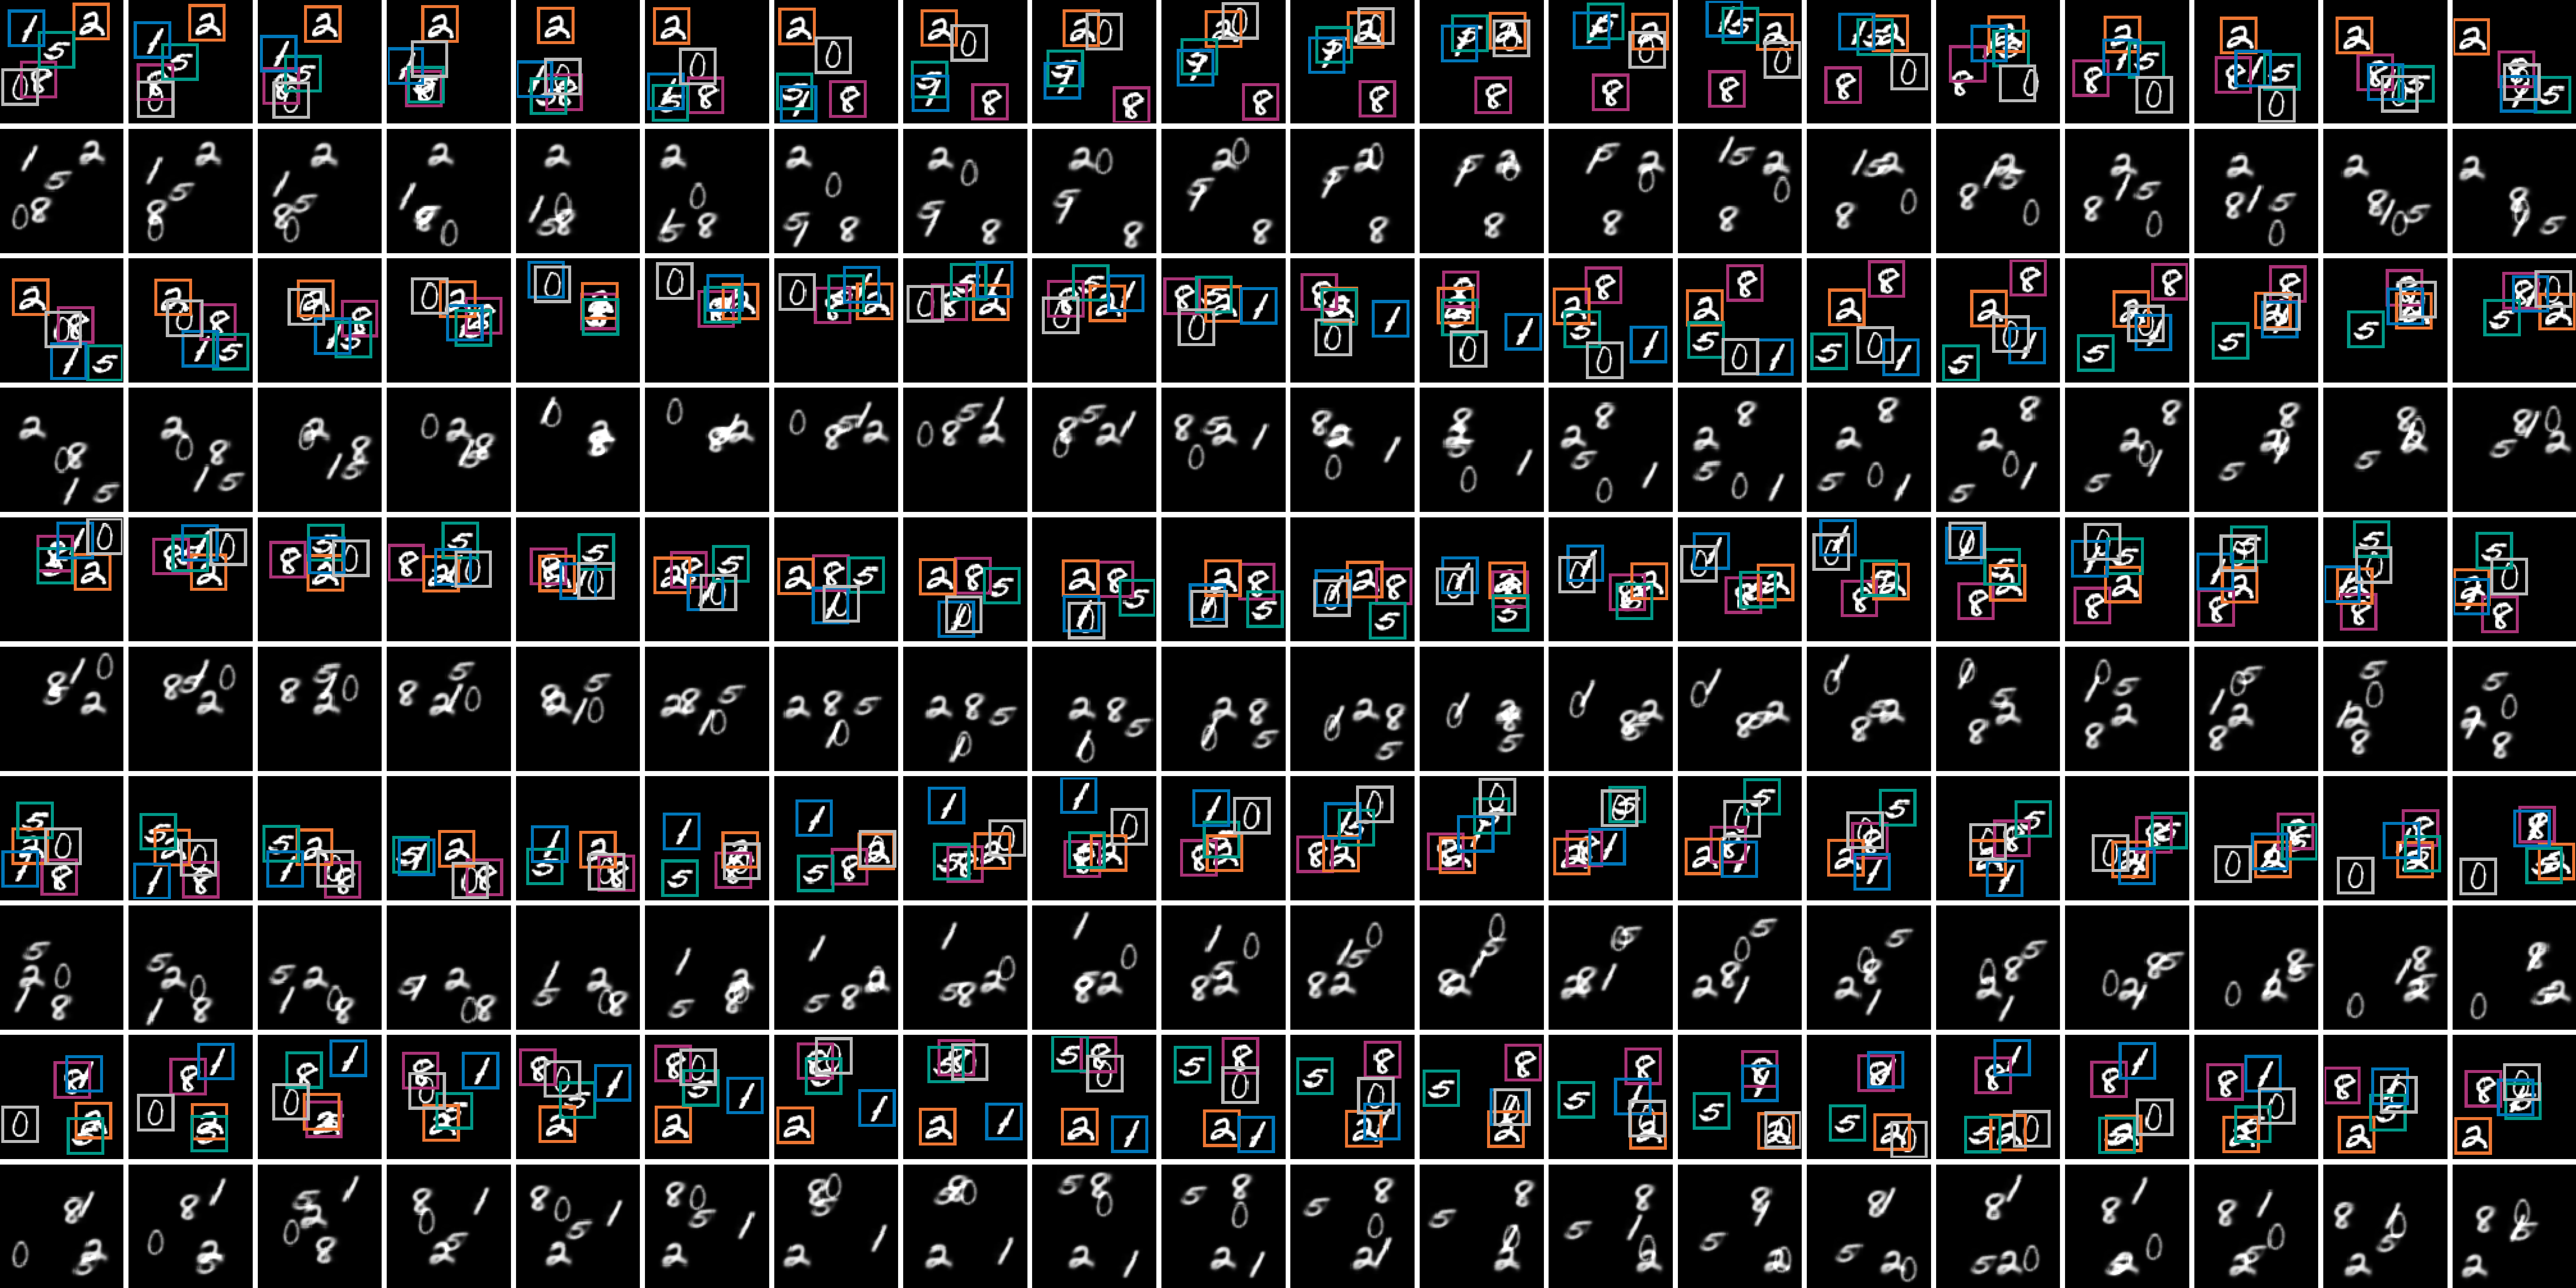
\includegraphics[width=170mm]{figures/T=100-D=5-2.pdf}
\caption{Full reconstruction for a video where $T=100, D=5$.}
\end{figure*}
\end{document}